\def\paperTitle{SAPA Capsule Project}
\def\paperSubTitle{Electric Stethoscope}

\documentclass[
	12pt,twoside,a4paper
]{report}

\usepackage{graphicx}
\usepackage[margin=1in]{geometry}
\usepackage{fancyhdr}
\usepackage[utf8]{inputenc}
\usepackage{etoc}
\usepackage{xcolor, soul}
\usepackage{listings}
\usepackage{amsmath}
\usepackage{lipsum}
\usepackage{pgfplots}
\usepackage{hyperref}
\usepackage{tikz}
\usepackage{circuitikz}
\usepackage[style=apa, backend=biber]{biblatex}

\addbibresource{refs.bib}
\DeclareLanguageMapping{english}{english-apa}

\sethlcolor{yellow}

\fancypagestyle{plain}{
	\fancyhf{}
	\fancyhead[l]{\paperTitle}
	\fancyhead[c]{\paperSubTitle}
	\fancyhead[r]{December 30, 2024}
	\fancyfoot[le, ro]{Page \thepage}
	\setlength{\headheight}{15pt}
	\renewcommand{\headrulewidth}{0.2pt}
	\renewcommand{\footrulewidth}{0.2pt}
}	

\thispagestyle{plain}

\renewcommand{\etocaftertitlehook}{\thispagestyle{plain}}
\renewcommand{\etocaftertochook}{\thispagestyle{plain}}

\begin{document}
\begin{center}
	
\includegraphics[width=0.4\textwidth]{assets/agu.png}

	\Huge
	\textbf{Abdullah Gül University}
	
	\vspace{0.3cm}
	Department of Electrical and Electronics Engineering

	\vspace{1cm}
	\Huge
	\textbf{\paperTitle}

	\vspace{0.3cm}
	\Huge
	\paperSubTitle{}

	\vspace{0.8cm}
	\large
	\vspace{0.5cm}
	\LARGE
	\vspace{1.5cm}
	\textbf{}
	\vfill
	\vspace{0.8cm}
	\Large
\end{center}

\begin{tabbing}
	\hspace*{1em}\= \hspace*{9em} \= \kill
	\> \textbf{Project Team:} \>  \\
	\> Barış DEMİRCİ \> agu@338.rocks \\
	\> Selin Nisa AKGÖL \> selinnisa.akgol@agu.edu.tr \\
	\> Nuri İNCEÖZ \> nuri.inceoz@agu.edu.tr \\
	\>  \\
	\> December 30, 2024 \\
\end{tabbing}

\tableofcontents

\chapter{Introduction}

\section{Background}
The stethoscope, a critical tool in medical diagnostics for nearly two centuries, has been a staple in physicians’ practices worldwide. With technological advancements, digital stethoscopes have emerged as modern alternatives, offering enhanced auscultation capabilities. These devices are cost-effective easy to use and capable of capturing both normal and abnormal breath sounds with high accuracy. This project aims to develop an electronic stethoscope system capable of acquiring and processing acoustic signals from various human body parts.

\section{Objective}
The primary goal is to design an electronic stethoscope system that acquires acoustic body sounds, converts them into digital signals, and transmits them to a computer for real-time monitoring and analysis. The system will include hardware and software components for:

\begin{itemize}
    \item Signal acquisition
    \item Amplification and filtering
    \item Digital conversion and transmission
    \item Real-time tracking via a graphical user interface (GUI)
\end{itemize}

\section{Scope}

\begin{itemize}
    \item The project involves designing custom amplification and filtering circuits without using commercial modules.
    \item Arduino will handle digital conversion and data transmission.
    \item Python will be used for GUI development, ensuring smooth signal monitoring and analysis.
\end{itemize}

\chapter{Hardware Development}

\section{Circuit Design \& Simulation}

\subsection{Electret Microphone Circuit}
First, tried to simulate the electrec microphone circuit using LTSpice. The circuit is shown in the figure below.

\begin{figure}[h]
	\centering
	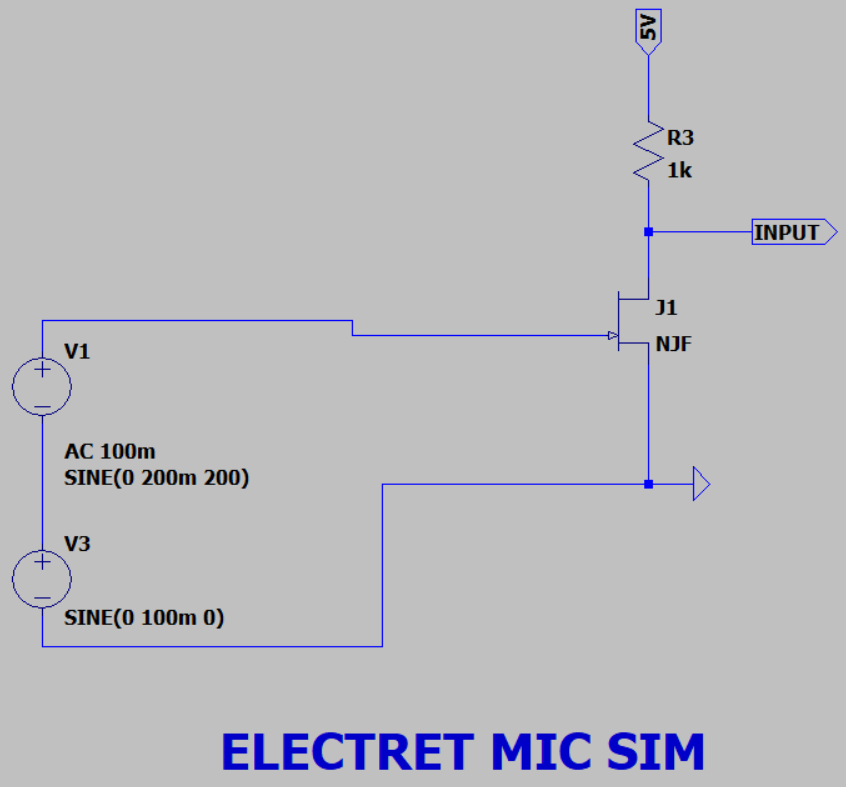
\includegraphics[width=0.6\textwidth]{assets/mic_circuit.png}
	\caption{Electret Microphone Circuit}
	\label{fig:mic_circuit}
\end{figure}

A 2-wire electrec microphone consists of one capacitor and one N-channel JFET. Using the circuit shown in Figure \ref{fig:mic_circuit}, we we able to acquire the voice signal from the microphone. Signal was too weak and too noisy to be used directly, so we needed to amplify and filter it.

\newpage
\thispagestyle{plain}

\subsection{Filter Circuit}

\subsubsection{High-Pass \& DC Filter}
Incoming signal was oscillating around 5V and had a lot of noise. We were planning to Arduino Uno for signal processing, so we needed to convert the signal to 0-5V range. We also needed to filter the noise. We designed a filter circuit using LTSpice.
\begin{figure}[h]
	\centering
	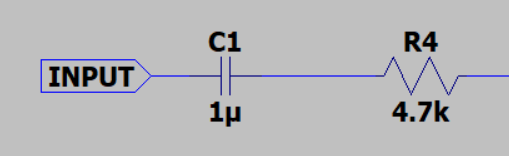
\includegraphics[width=0.6\textwidth]{assets/high-pass.png}
	\caption{High-Pass Filter Circuit}
	\label{fig:hp_filter_circuit}
\end{figure}

Used a passive high-pass filter setup as shown in Figure \ref{fig:hp_filter_circuit} for both filtering DC offset and low frequency noise. The cutoff frequency can be calculated using the formula:
\begin{equation}\label{eq:filter_cutoff}
	f_c = \frac{1}{2\pi RC}
\end{equation}
In our case, we used R = $4.7k\Omega$ and C = $1\mu$F, so the cutoff frequency was $33.8$Hz. This filter was able to filter out the DC offset and low frequency noise.

\subsubsection{Low-Pass Filter}

\begin{figure}[h]
	\centering
	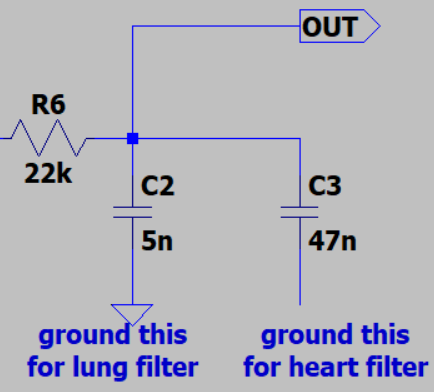
\includegraphics[width=0.5\textwidth]{assets/low-pass.png}
	\caption{Low-Pass Filter Circuit}
	\label{fig:lp_filter_circuit}
\end{figure}

Again, used a passive low-pass filter setup as shown in Figure \ref{fig:lp_filter_circuit} for filtering high frequency noise. The cutoff frequency can be calculated using the formula \ref{eq:filter_cutoff}. In our case, we used R = $22k\Omega$ and C = $5$nF for lung, C = $47$nF for heart, so the cutoff frequency was $153$Hz for heart and $1446$Hz for lung. This filter was able to filter out the high frequency noise.

\newpage
\thispagestyle{plain}

\subsection{Amplifier Circuit}

\begin{figure}[h]
	\centering
	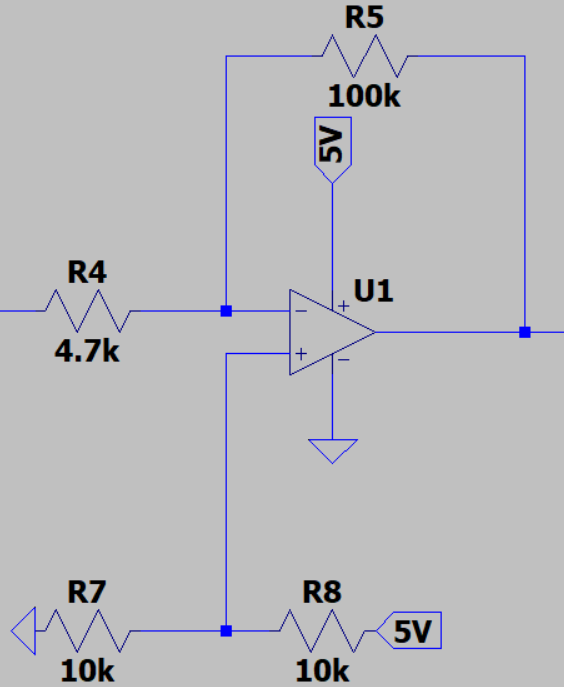
\includegraphics[width=0.6\textwidth]{assets/amplifier.png}
	\caption{Amplifier Circuit}
	\label{fig:amplifier_circuit}
\end{figure}

We used an inverting op-amp circuit for amplifying the signal, adding 2.5V DC bias, and inverting the signal to its original state (because the signal was inverted by the electrec mic). The gain of the amplifier can be calculated using the formula:

\begin{equation}\label{eq:amplifier_gain}
	G = -\frac{R_f}{R_1}
\end{equation}

In our case, we used $R_1 = 4.7k\Omega$ and $R_f = 100k\Omega$, so the gain was approximately $-20$. This amplifier was able to amplify the signal to a usable level. For DC bias, we used a voltage divider ciruit to get 2.5V and connected it to the non-inverting input of the op-amp, which made our signal oscillate around 2.5V.

\newpage
\thispagestyle{plain}

\subsection{Final Circuit}

After connecting everything together, the final circuit looked like this:

\begin{figure}[h]
	\centering
	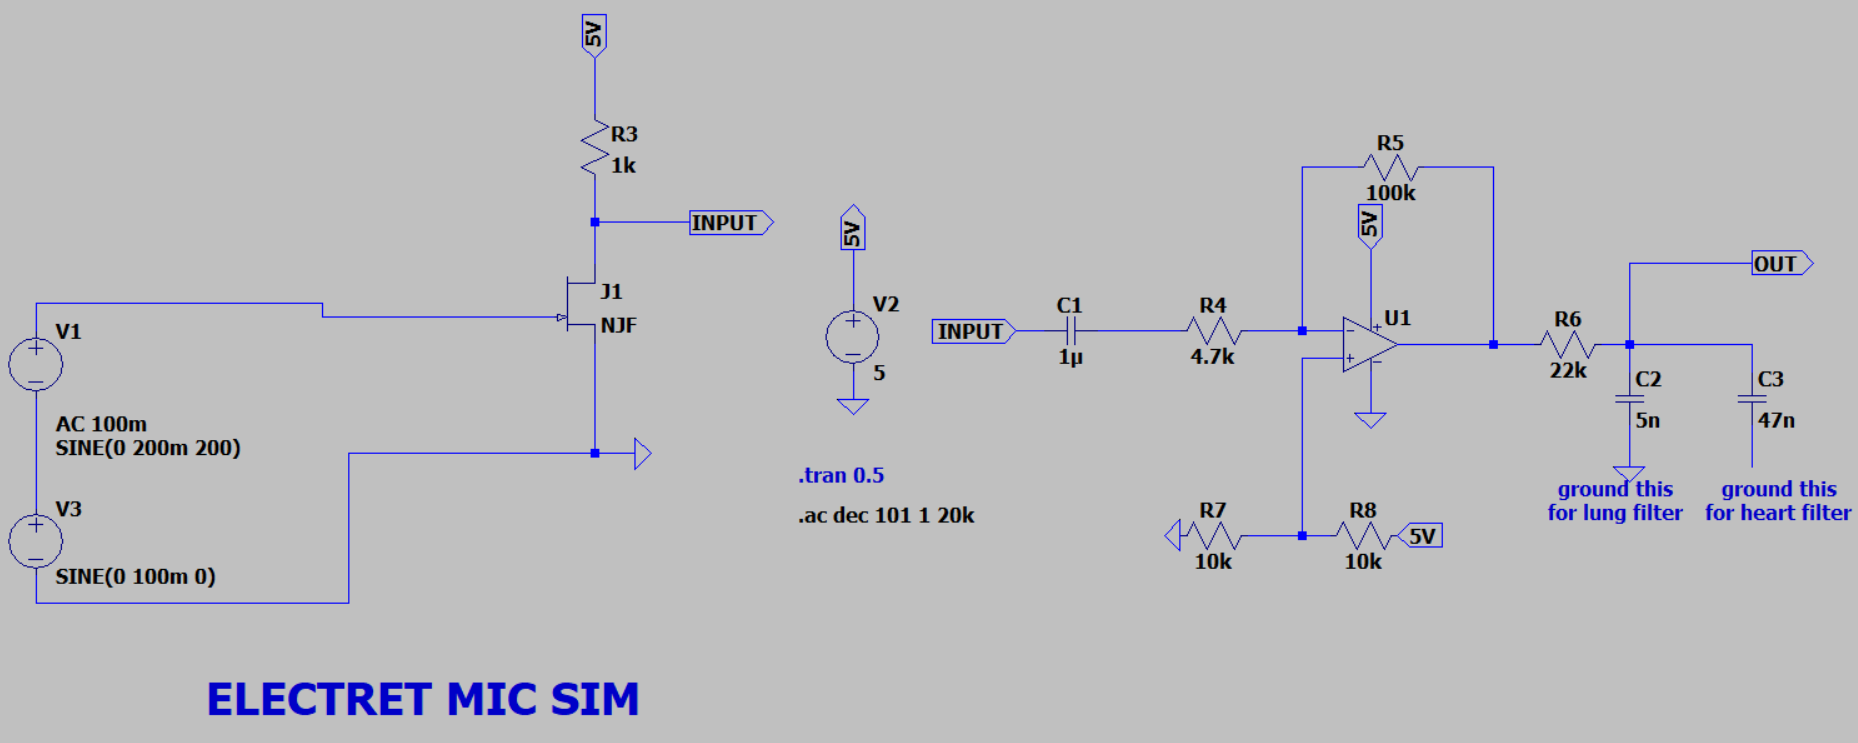
\includegraphics[width=1\textwidth]{assets/final-circuit.png}
	\caption{Final Circuit}
	\label{fig:final_circuit}
\end{figure}

To test the circuit, we used a function generator to simulate the electrec microphone signal. We were able to get the signal from the microphone, amplify it, and filter it successfully. After building the circuit we ran an AC simulation on LTSpice and checked the cutoff frequencies.

\begin{table}[h]
	\begin{tabular}{l|l|l|}
		\cline{2-3}
		                                                & \textbf{Analytical Cutoff Frequency} & \textbf{Simulation Result} \\ \hline
		\multicolumn{1}{|l|}{\textbf{High-Pass}}        & 33.8Hz                               & 26.7Hz                     \\ \hline
		\multicolumn{1}{|l|}{\textbf{Low-Pass (Heart)}} & 153Hz                                & 205Hz                      \\ \hline
		\multicolumn{1}{|l|}{\textbf{Low-Pass (Lung)}}  & 1466Hz                               & 1530Hz                     \\ \hline
	\end{tabular}
	\caption{Cutoff Frequencies}
	\label{tab:cutoff_frequencies}
\end{table}

According to \textcite{Debbal2020}, these frequencies are suitable for heartbeat detection and according to \textcite{Gross2000}, these frequencies are suitable for lung sound detection.

\newpage
\thispagestyle{plain}

\section{Prototype Design}

\subsection{Breadboard Prototype}
We have built the circuit in Figure \ref{fig:final_circuit} on a breadboard and measured output voltages using an oscilloscope.

\begin{figure}[h]
	\centering
	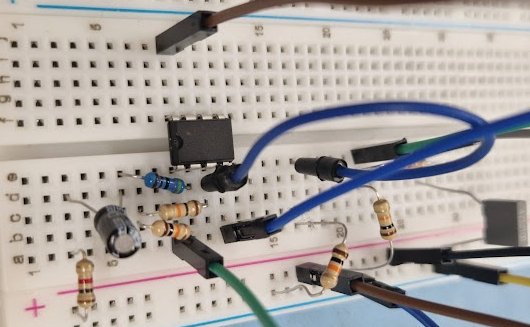
\includegraphics[width=0.7\textwidth]{assets/breadboard.png}
	\caption{Breadboard Prototype}
	\label{fig:breadboard_prototype}
\end{figure}

\begin{figure}[h]
	\centering
	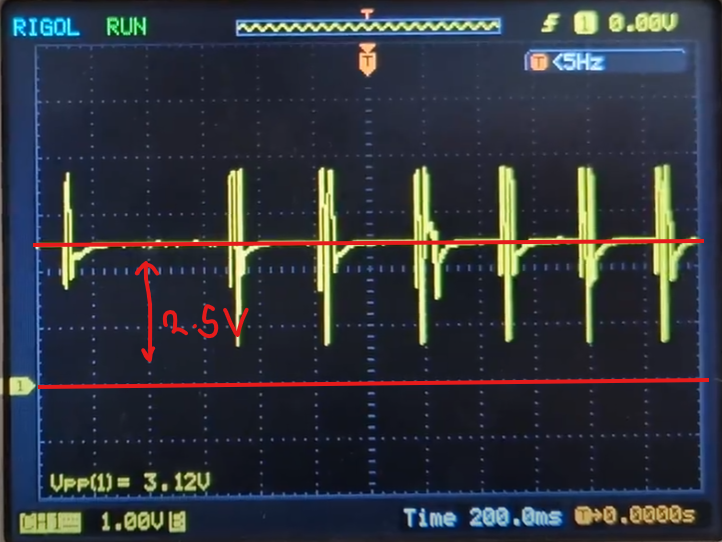
\includegraphics[width=0.5\textwidth]{assets/breadboard-output.png}
	\caption{Breadboard Prototype Output}
	\label{fig:breadboard_prototype_output}
\end{figure}

Output was exactly as expected. We were able to get the signal from the microphone, amplify it, give 2.5V DC bias, and filter it successfully.

\newpage
\thispagestyle{plain}

\subsection{Pertinax Board Design}

After making sure that the circuit works as expected, we soldered the circuit parts to perforated pertinax board as shown in Figure \ref{fig:pertinax_board_design}.

\begin{figure}[h]
	\centering
	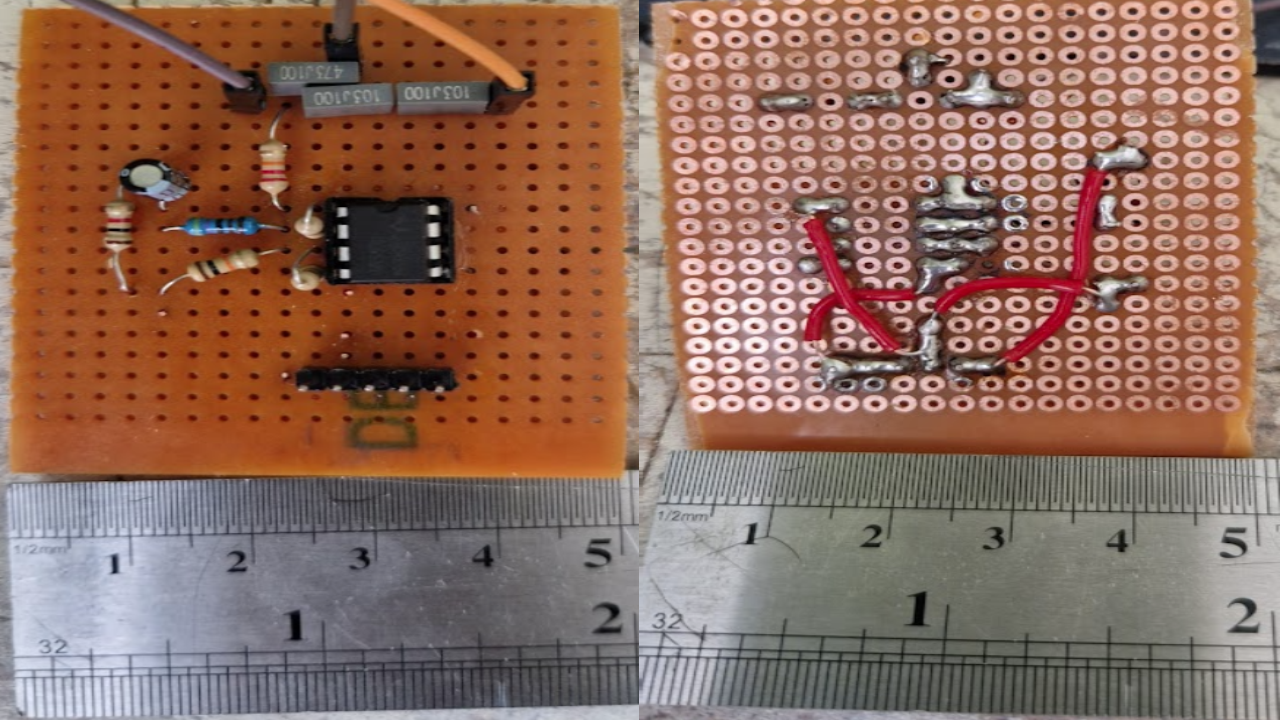
\includegraphics[width=1\textwidth]{assets/pertinax-design.png}
	\caption{Pertinax Board Design}
	\label{fig:pertinax_board_design}
\end{figure}

\newpage
\thispagestyle{plain}

\subsection{Casing Design}

We designed a casing for the prototype using SolidWorks. Casing has required pin headers for microphone, Arduino, and power supply connections.

\begin{figure}[h]
	\centering
	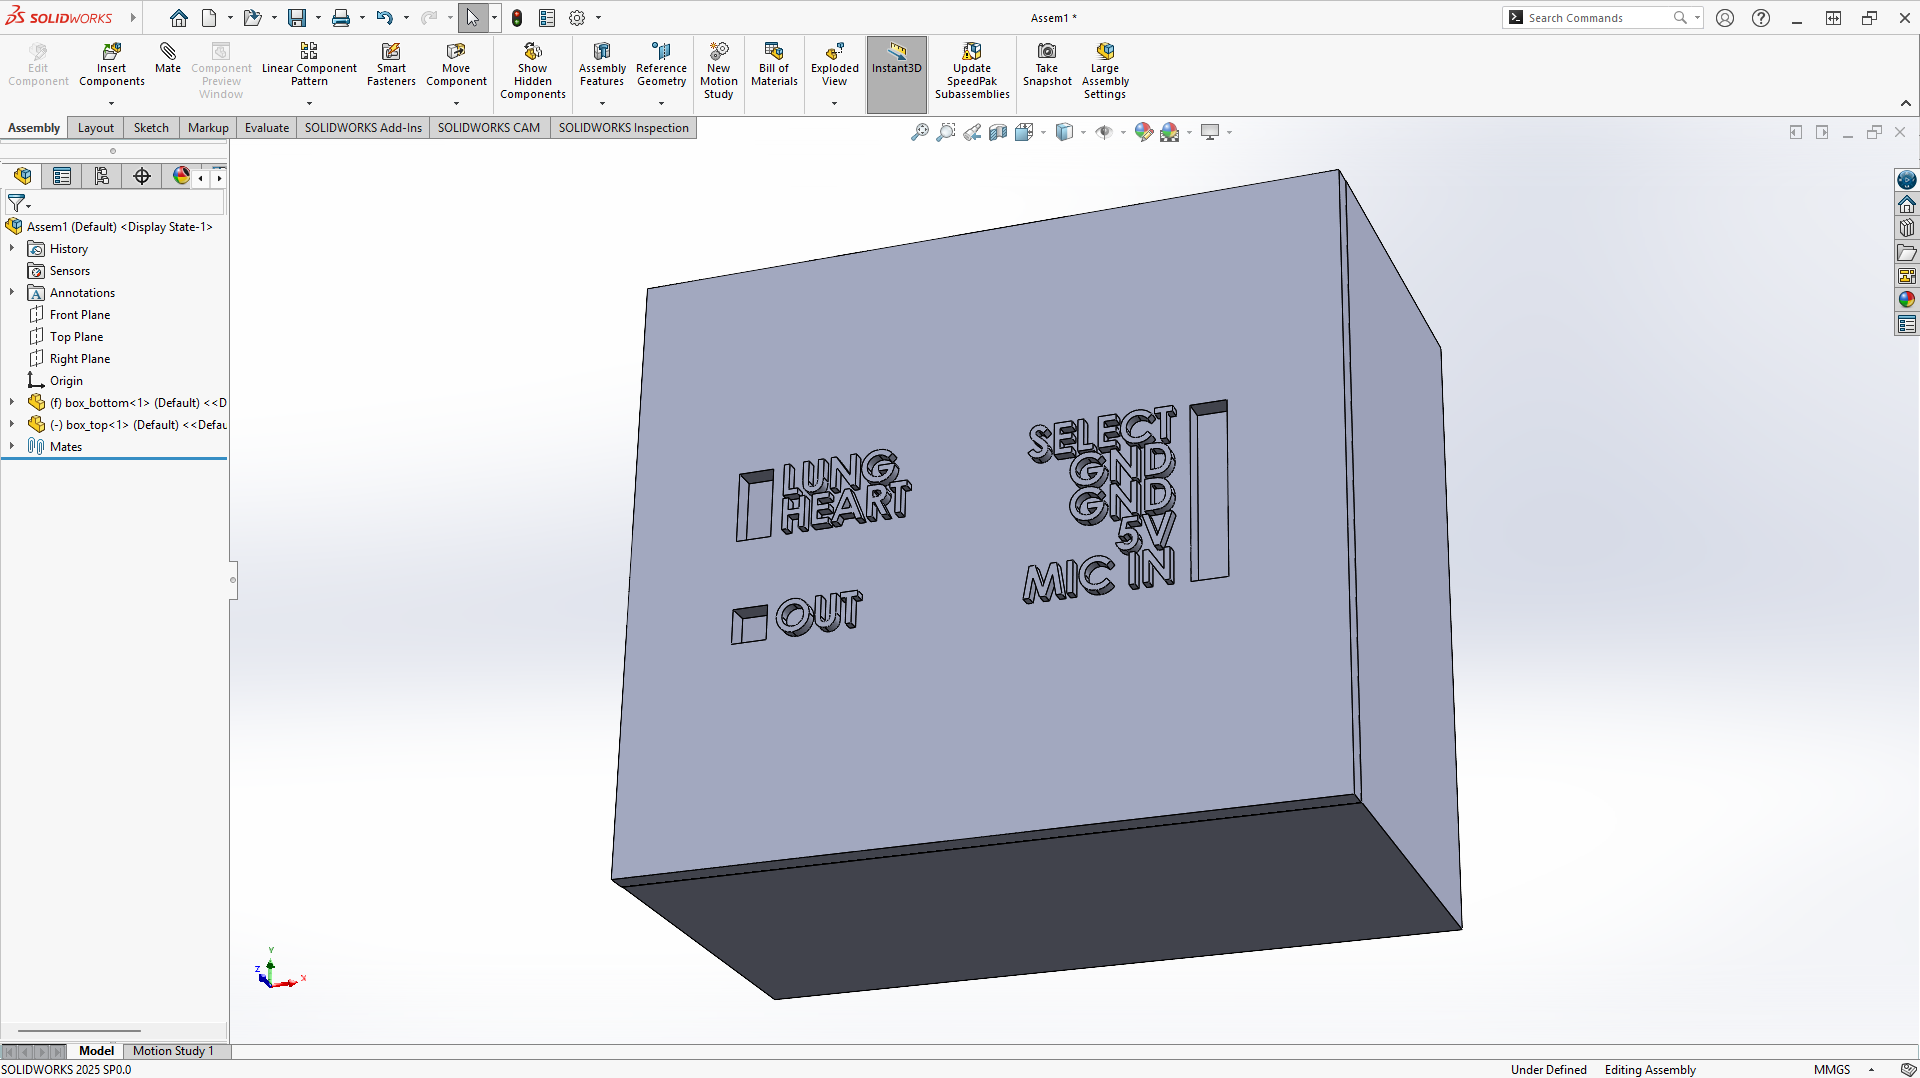
\includegraphics[width=0.7\textwidth]{assets/3d-design.png}
	\caption{Casing Design}
	\label{fig:casing_design}
\end{figure}

\begin{figure}[h]
	\centering
	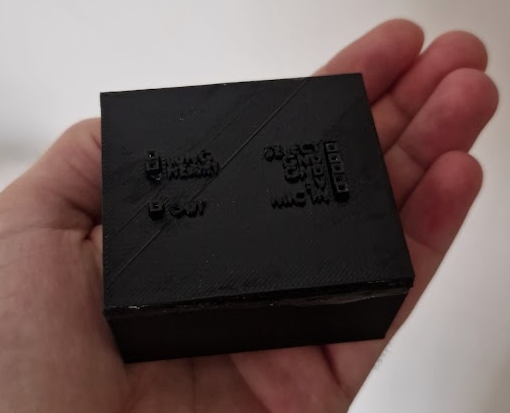
\includegraphics[width=0.5\textwidth]{assets/3d-design-printed.png}
	\caption{Casing Design Printed}
	\label{fig:casing_design_printed}
\end{figure}

Our first prototype is worked as expected so we decided to use it as our final prototype. By putting the prototype in the casing, we completed the hardware development phase.

\chapter{Software Development}

\section{Arduino Code}\label{sec:arduino_code}

We used an Arduino Uno for signal transmission. It already has its own 10-bit 0-5V ADC for analog signal transmission. We already made the necessary signal processing on the hardware side, our signal oscillates around 2.5V and has a range of 0-5V. We can start to read the signal using Arduino without any problem or any signal loss.


Before starting to measure the analog signal, we measured the reading speed using the following benchmark code in order to decide what sampling rate we should use:

\begin{lstlisting}[language=C++, caption=Analog Read Benchmark Code, label=lst:analog_read_benchmark]
void loop() {
    unsigned long start = micros();
    analogRead(A0);
    unsigned long end = micros();
    Serial.println(end - start);
}
\end{lstlisting}

The code reads the analog signal from pin A0 and prints the time taken to read the signal in microseconds. We used this code to measure the analog signal reading speed of the Arduino Uno. The average time taken to read the analog signal was 112$\mu$s. This means that the Arduino Uno can read the analog signal at a rate of 8.9kHz. This is more than enough for our project, as the maximum frequency of the signal we are trying to measure is 2kHz.

According to \textcite{Wikiedia-NyquistShannon2024}, Nyquist-Shannon Sampling Theorem says the minimum sampling rate should be twice the maximum frequency of the signal. So, we need a minimum sampling rate of 4kHz, but more is better.

\newpage
\thispagestyle{plain}

Arduino Uno can read the analog signal at a rate of 8.9kHz, which is more than enough for our project but for stability (because read speed vary around 108$\mu$s to 116$\mu$s according to our benchmarks), we decided to use a sampling rate of 8kHz (125$\mu$s, more than benchmark average). To achieve this, we used the following code:

\begin{lstlisting}[language=C++, caption=Arduino Code for 8kHz Sampling Rate, label=lst:arduino_code]
void loop() {
    unsigned long startedAt = micros();

    // Send the sensor value to the serial port
    int sensorValue = analogRead(analogPin);
    Serial.println(sensorValue);

    unsigned long endedAt = micros();
    unsigned long timeTook = endedAt - startedAt;

    // 125us = 8kHz sampling rate
    unsigned long timeRemaining = 125 - timeTook;

    // Wait for the remaining time
    // this approach will give us 8kHz sampling rate in theory
    // But in practice, it may not be exactly 8kHz 
    // but it is good enough for our purposes
    if (timeRemaining > 0) {
        delayMicroseconds(timeRemaining);
    }
}
\end{lstlisting}

This code reads the analog signal from pin A0, prints the signal value to the serial port, and waits for the remaining time to achieve an 8kHz sampling rate. This code will give us an 8kHz sampling rate in theory, but in practice, it may not be exactly 8kHz. However, it is good enough for our purposes.

\newpage
\thispagestyle{plain}

While this code prints the analog signal value to the serial port at 8kHz sampling rate, we used a Python script to read the serial port. Sometimes, Python cannot read the serial data correctly because this process is an asynchronous process. Maybe Arduino sends half of the data before Python is ready to read it. To prevent this, we can use starting and ending characters for the serial communication and keep a buffer in Python. We used the following code for this purpose:

\begin{lstlisting}[language=C++, caption=Arduino Code with Start and End Characters, label=lst:arduino_code_start_end]
const int analogPin = A0;

// Define the starting and ending characters 
// for the serial communication. 
// Sometimes python cannot read the serial data incorrectly. 
// To prevent this, we can use starting and ending characters.
const String startingChar = "S";
const String endingCar = "E";

void loop() {
    unsigned long startedAt = micros();

    int sensorValue = analogRead(analogPin);
    
    // Print the value with starting and ending characters
    Serial.print(startingChar);
    Serial.print(sensorValue);
    Serial.println(endingCar);

    // On serial port: 
    // SxxxxE -> S: Start, E: End, xxxx: Sensor Value
    // Example
    // S338E -> S: Start, E: End, 338: Sensor Value

    unsigned long endedAt = micros();
    unsigned long timeTook = endedAt - startedAt;

    // 125us = 8kHz sampling rate
    unsigned long timeRemaining = 125 - timeTook;

    // Wait for the remaining time
    // this approach will give us 8kHz sampling rate in theory
    // But in practice, it may not be exactly 8kHz 
    // but it is good enough for our purposes
    if (timeRemaining > 0) {
        delayMicroseconds(timeRemaining);
    }
}
\end{lstlisting}

This code prints the analog signal value to the serial port with starting and ending characters. This way, we can prevent Python from reading the serial data incorrectly.

\newpage
\thispagestyle{plain}

\section{Python Code}

We used Python to read the serial port, process the analog signal and show the real-time signal on a GUI. As we mentioned in Section \ref{sec:arduino_code}, Arduino Code, we used starting and ending characters for the serial communication. We used these characters to prevent Python from reading the serial data incorrectly. We used the following code to read the serial port:

\begin{lstlisting}[language=Python, caption=Python Code to Read Serial Port, label=lst:python_code_read_serial]
# Read data from serial port. Read Arduino code for more details
data_buffer = ""
while ser.in_waiting > 0:
    try:
        char = ser.read().decode("utf-8")
        data_buffer += char

        if "E" in data_buffer and "S" in data_buffer:
            try:
                start_index = data_buffer.index("S")
                end_index = data_buffer.index("E")
                value_str = data_buffer[start_index + 1 : end_index]
                if value_str.isdigit():
                    analog_value = int(value_str)

                    # Normalize and zero center because 
                    # most of the dsp functions 
                    # require zero centered data
                    normalized = (
                        (analog_value / 1024.0) * 5.0
                    ) - 2.5

                    # Append the normalized value to the list
                    # So that we can plot it later
                    analog_data.append(normalized)
                    time_data.append(time.time())

                    while time_data and (time_data[-1] - time_data[0] > 5):
                        time_data.popleft()
                        analog_data.popleft()
            except ValueError:
                pass
            data_buffer = ""

    except UnicodeDecodeError:
        data_buffer = ""
    except Exception:
        data_buffer = ""
\end{lstlisting}

\newpage
\thispagestyle{plain}

With this code, we read the serial port and process the analog signal. We normalized the analog signal to be zero-centered because most of the digital signal processing functions require zero-centered data. We also kept the last 5 seconds of the data in the list to plot it later.

While these codes are the most important parts of the software development, we also developed a GUI to show the real-time signal which we are not mentioning the code here. The GUI is developed using the tkinter and matplotlib library. You can always check the full code from the GitHub repository of the project, which is given in Appendix \ref{sec:appendix_a}.

\begin{figure}[h]
	\centering
	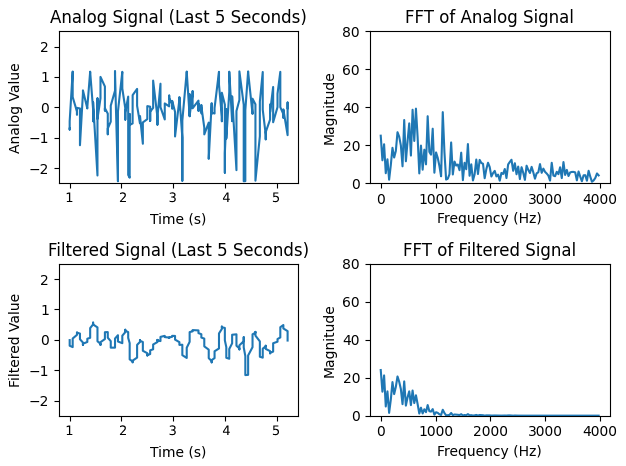
\includegraphics[width=0.8\textwidth]{assets/plots.png}
	\caption{GUI of the Project}
	\label{fig:gui}
\end{figure}

\begin{figure}[h]
	\centering
	\begin{minipage}{0.5\textwidth}
		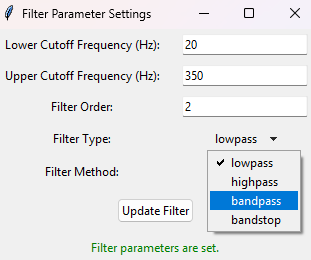
\includegraphics[width=0.9\textwidth , height=0.2\textheight]{assets/filter-type-selector.png}
		\caption{Filter Type Selector}
		\label{fig:gui-filter-type-selector}
	\end{minipage}%
	\begin{minipage}{0.5\textwidth}
		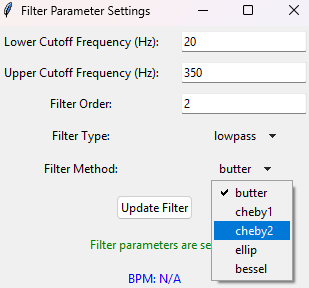
\includegraphics[width=0.9\textwidth , height=0.2\textheight]{assets/filter-method-selector.png}
		\caption{Filter Method Selector}
		\label{fig:gui-filter-method-selector}
	\end{minipage}
\end{figure}

\chapter{Conclusion}

The development of the electronic stethoscope demonstrates the integration of electronics, software, and medical knowledge to create a modern diagnostic tool. With its ability to capture, process, and analyze body sounds, this device provides a valuable addition to healthcare diagnostics. Further improvements in signal processing and hardware miniaturization could make this tool indispensable for clinicians.

This project demonstrated how easy to design a digital stethoscope using off-the-shelf components. The device was able to capture and process body sounds, and the results were displayed on a computer screen. With further development, the device could be used for real-time diagnosis and monitoring of patients.


\newpage
\thispagestyle{plain}

\chapter*{Appendix}
\addcontentsline{toc}{chapter}{Appendix}

\section*{Appendix A: Github Repositoy}\label{sec:appendix_a}
\addcontentsline{toc}{section}{Github Repository}
\url{https://github.com/dotrocks/sapa-project-electric-stethoscope}

\printbibliography{}
\addcontentsline{toc}{chapter}{Bibliography}
\end{document}
